\begin{tikzpicture}[execute at end picture={
    % \draw (current bounding box.south west)
    %     grid [step=0.5cm] (current bounding box.north east);
}]
    \node[inner sep=0pt, above right] (screen) at (0,0) {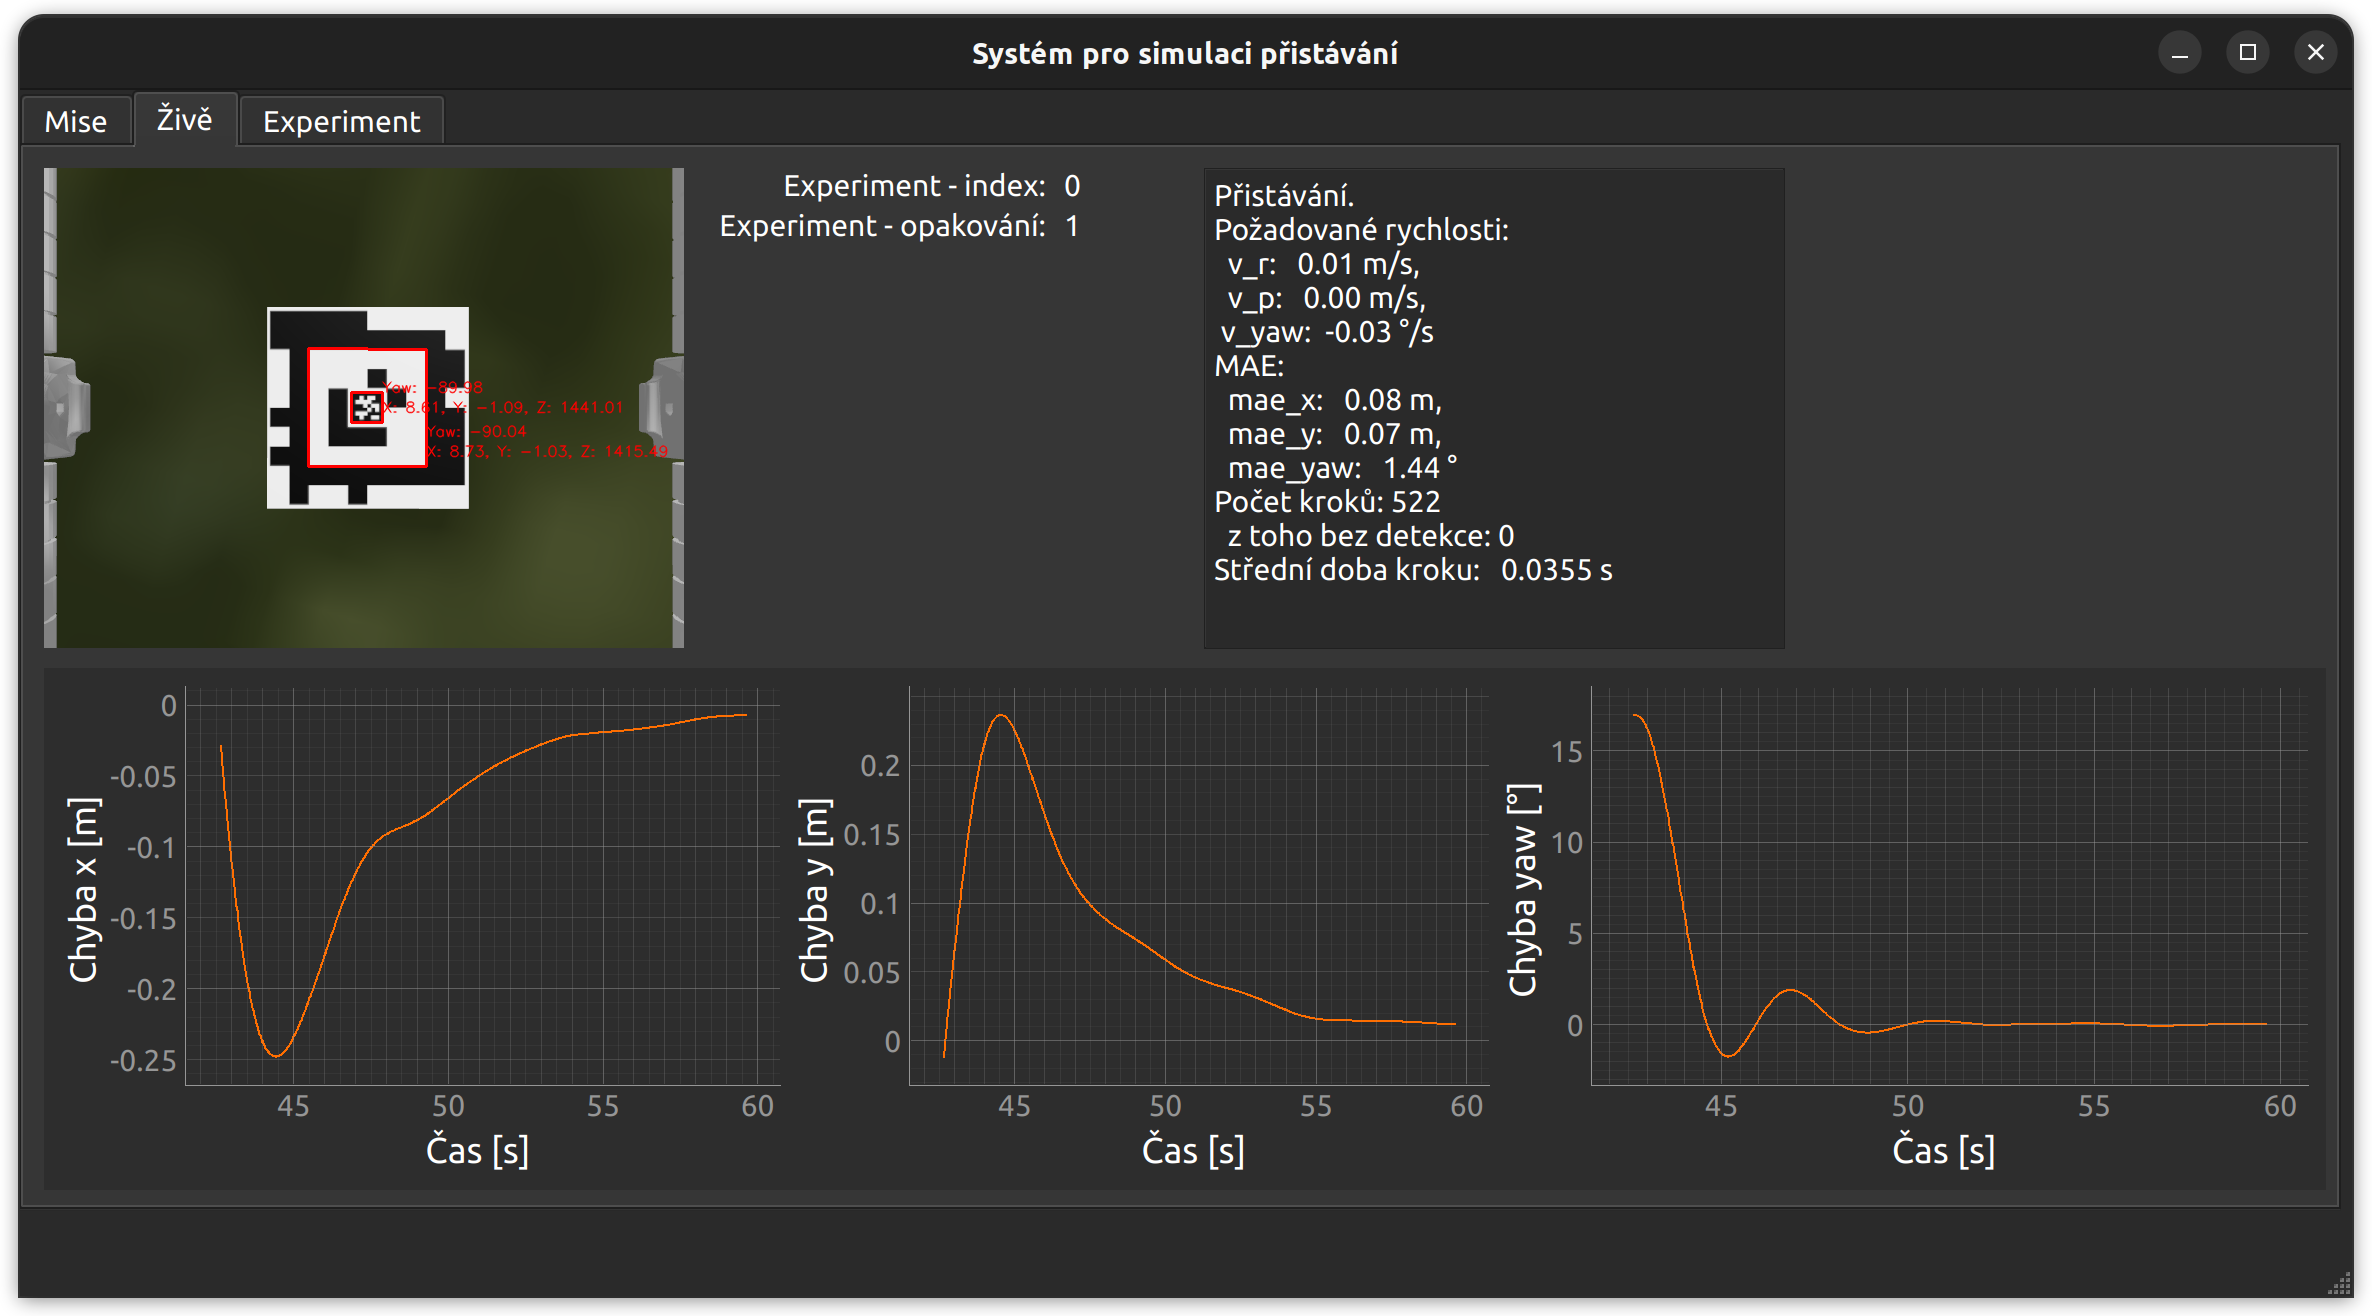
\includegraphics[width=\textwidth]{gui/live (2).png}};

    \node[draw, above right, minimum height=3cm, minimum width=4.05cm, color=red, line width=1pt, pin={[pin={[pin distance=0cm,draw,circle,node font=\tiny,pin edge={red}]left:2},pin distance=2.1cm, pin edge={red}]75:Pohled kamery}] (kamera) at (0.25,4.2) {};

    \node[draw, above right, minimum height=3.2cm, minimum width=14.5cm, color=cyan, line width=1pt, pin={[pin={[pin distance=0cm,draw,circle,node font=\tiny,pin edge={cyan}]left:5},pin distance=1.2cm, pin edge={cyan}]below:Grafy chyb}] (grafy) at (0.25,0.75) {};
    \node[draw, above right, minimum height=0.5cm, minimum width=2.4cm, color=blue, line width=1pt, pin={[pin={[pin distance=0cm,draw,circle,node font=\tiny,pin edge={blue}]left:3},pin distance=1.6cm, pin edge={blue}]80:Informace o experimentu}] (expInfo) at (4.45,6.7) {};
    \node[draw, above right, minimum height=3cm, minimum width=3.75cm, color=orange, line width=1pt, pin={[pin={[pin distance=0cm,draw,circle,node font=\tiny,pin edge={orange}]left:4},pin distance=2cm, pin edge={orange}]55:Stav algoritmu}] (alg) at (7.55,4.15) {};

    \node[draw, above right, minimum height=0.47cm, minimum width=2.77cm, color=green, line width=1pt, pin={[pin={[pin distance=0cm,draw,circle,node font=\tiny,pin edge={green}]above:1},pin distance=1cm, pin edge={green}]above:Výběr obrazovky}] (zalozky) at (0.06,7.25) {};
\end{tikzpicture}